%%%%%%%%%%%%%%%%%%%%%%%%%%%%%%%%%%%%%%%%%%%%%%%%%%%%%%%%%%%%%%%%%%%%%%%%%%%%
%% Author template for INFORMS Journal on Data Science (ijds) [interim solution; new styles under construction]
%% Mirko Janc, Ph.D., INFORMS, mirko.janc@informs.org
%% ver. 0.91, March 2015 - updated November 2020 by Matthew Walls, matthew.walls@informs.org
%%%%%%%%%%%%%%%%%%%%%%%%%%%%%%%%%%%%%%%%%%%%%%%%%%%%%%%%%%%%%%%%%%%%%%%%%%%%
\documentclass[ijds,nonblindrev]{informs-ijds}


%%% temporary functions - remove for final
\usepackage{soul}
%%% uncomment below to hide strike through
\makeatletter
\renewcommand\st[1]{\@bsphack\@esphack}%
\makeatother
\usepackage{xcolor}
\newcommand{\ET}[1]{\textcolor{purple}{#1}}

%%%%%%%

\OneAndAHalfSpacedXI
%%\OneAndAHalfSpacedXII % Current default line spacing
%%\DoubleSpacedXII
%%\DoubleSpacedXI

% Private macros here (check that there is no clash with the style)

% Natbib setup for author-year style
\usepackage{natbib}
 \bibpunct[, ]{(}{)}{,}{a}{}{,}%
 \def\bibfont{\small}%
 \def\bibsep{\smallskipamount}%
 \def\bibhang{24pt}%
 \def\newblock{\ }%
 \def\BIBand{and}%



%% Setup of theorem styles. Outcomment only one.
%% Preferred default is the first option.
\TheoremsNumberedThrough     % Preferred (Theorem 1, Lemma 1, Theorem 2)
%\TheoremsNumberedByChapter  % (Theorem 1.1, Lema 1.1, Theorem 1.2)
\ECRepeatTheorems

%% Setup of the equation numbering system. Outcomment only one.
%% Preferred default is the first option.
\EquationsNumberedThrough    % Default: (1), (2), ...
%\EquationsNumberedBySection % (1.1), (1.2), ...

% For new submissions, leave this number blank.
% For revisions, input the manuscript number assigned by the on-line
% system along with a suffix ".Rx" where x is the revision number.
\MANUSCRIPTNO{IJDS-0001-1922.65}

%%%%%%%%%%%%%%%%
\begin{document}
%%%%%%%%%%%%%%%%

% Outcomment only when entries are known. Otherwise leave as is and
%   default values will be used.
%\setcounter{page}{1}
%\VOLUME{00}%
%\NO{0}%
%\MONTH{Xxxxx}% (month or a similar seasonal id)
%\YEAR{0000}% e.g., 2005
%\FIRSTPAGE{000}%
%\LASTPAGE{000}%
%\SHORTYEAR{00}% shortened year (two-digit)
%\ISSUE{0000} %
%\LONGFIRSTPAGE{0001} %
%\DOI{10.1287/xxxx.0000.0000}%

% Author's names for the running heads
% Sample depending on the number of authors;
% Enter authors following the given pattern:
\RUNAUTHOR{Tanaka, Leung, and Cook}

% Title or shortened title suitable for running heads. 
% Enter the (shortened) title:
\RUNTITLE{Incorporating statistical thinking into visualisation practices for decision-making}

% Full title. Sample:
% \TITLE{Bundling Information Goods of Decreasing Value}
% Enter the full title:
\TITLE{Incorporating statistical thinking into visualisation practices for decision-making in operational management}

% Block of authors and their affiliations starts here:
% NOTE: Authors with same affiliation, if the order of authors allows,
%   should be entered in ONE field, separated by a comma.
%   \EMAIL field can be repeated if more than one author
\ARTICLEAUTHORS{%
\AUTHOR{Emi Tanaka}
\AFF{Department of Econometrics and Business Statistics, Monash University, Melbourne, VIC 3800, \EMAIL{emi.tanaka@monash.edu}} %, \URL{}}
\AUTHOR{Jessica Wai Yin Leung}
\AFF{Department of Econometrics and Business Statistics, Monash University, Melbourne, VIC 3800, \EMAIL{jessica.leung@monash.edu}}
\AUTHOR{Dianne Cook}
\AFF{Department of Econometrics and Business Statistics, Monash University, Melbourne, VIC 3800, \EMAIL{dicook@monash.edu}} %, \URL{}}
% Enter all authors
} % end of the block

\ABSTRACT{%

% Enter your abstract
}%

% Fill in data. If unknown, outcomment the field
\KEYWORDS{statistical graphics; graphical inference; visual inference; grammar of graphics; visual encoding; reproducibility} %\HISTORY{This paper ....}

\maketitle
%%%%%%%%%%%%%%%%%%%%%%%%%%%%%%%%%%%%%%%%%%%%%%%%%%%%%%%%%%%%%%%%%%%%%%

% Samples of sectioning (and labeling) in MNSC
% NOTE: (1) \section and \subsection do NOT end with a period
%       (2) \subsubsection and lower need end punctuation
%       (3) capitalization is as shown (title style).
%
%\section{Introduction.}\label{intro} %%1.
%\subsection{Duality and the Classical EOQ Problem.}\label{class-EOQ} %% 1.1.
%\subsection{Outline.}\label{outline1} %% 1.2.
%\subsubsection{Cyclic Schedules for the General Deterministic SMDP.}
%  \label{cyclic-schedules} %% 1.2.1
%\section{Problem Description.}\label{problemdescription} %% 2.

% Text of your paper here

\section{Introduction}

\citet{basole2021} demonstrate that visualisation can aid or mislead depending on its use -- we strongly agree that visualisation is indeed a double-edged sword that can uncover unexpected information and communicate information effectively but poor practices can lead to misinterpretation or over-emphasis of a feature in the plot. Applying the Gestalt laws, \citet{basole2021} illustrate the importance of choosing the appropriate chart elements. We concur that appropriate visual encoding is vital for enhancing the visual decoding accuracy of a graph, however there is more discussion needed on the visual encoding process and the incorporation of statistical thinking when working with visual displays of data. These two points form the focus of this commentary. %using rigorous assessment frameworks for inferences based on statistical graphics -- we elaborate on these matters in Sections~\ref{sec:plotdesign} and \ref{sec:visinf}, respectively. In particular, we offer statistical perspectives in data visualisation and emphasise the need for rigour in both the production and the interpretations of plots. We conclude with future directions in Section~\ref{sec:conclude}. 

It is motivating to see that \citet{basole2021} provide an instructive framework on the goal, benefits and challenges of visualisation, considering the iterative and evolving nature of graphical process, and the varying needs and challenges presented at different stages of empirical operational management research. We find the discussion highlighting the continuing and emerging concerns in terms of data security and data ethics and how they relate to visualisation intriguing and timely. The strategies and examples to mitigate these concerns covered in the paper also provided significant insights into how and to what extent institutions should incorporate similar measures.

\section{Visualising encoding choices} \label{sec:plotdesign}

Encoding refers to the process and choices made for displaying the data in a graph. Decoding describes the process of interpreting or perceiving the information from the graph. Different encoding approaches lead to differences in decoding information. \citet{basole2021} use the Gestalt principles of perceptual organization to demonstrate misrepresentations by inclusion and omission on a graph. We agree that this is highly pertinent to enhance the visual decoding accuracy of a graph and that the discussion can be extended to include the choices in the visual encoding process. In a visual encoding process, retinal variables, such as position, size, shape, color hue, color intensity, orientation, texture, and motion, are used to represent different information in the data \citep{bertin1983semiology, munzner2014visualization}. \cite{graphworkflow} provides a website with convenient explanation with a compact diagram to illustrate such choices. The encoding process was formalised into a grammar by \citealp{Wilkinson2005-oz} that specifies the mapping of the data variables to retinal variables. The grammar was extended and implemented in the \texttt{ggplot2} R-package \citep{ggplot2}. The connection with statistics is tightened because the mapping requires that data is organised as ``tidy data'' \citep{tidyr}, where variables are in columns and observations are in rows. For example, the data used in Figure~3 from \citet{basole2021} contains the variables: state, coverage, readmission rate and cancer screening percentage, and additionally two spatial variables ($x$, $y$) specifying state tile location. These variables are mapped as follows to produce the visual display: $x$ to the $x$-axis (like longitude), $y$ to the $y$-axis (like latitude), size to coverage, using a circle geometry, and color to readmission rate (left plot), or cancer screening percentage (right plot).

\citet{basole2021} use Figure~3 to assert that ``In this depiction, one can discern that states with highly integrated care also tend to have (i.e. are predictive of) higher cancer screening rates and lower 30-day hospital readmissions.'' --  we interpret integrated care to mean coverage here. {\em We disagree with this statement, and feel that the authors may have misinterpreted the plot.} A better visual encoding for examining association between two variables is the humble scatter plot, where coverage is mapped to the $x$-axis and either the readmission rate or cancer screening percentage is mapped to the $y$-axis, as shown here in Figure~\ref{fig:fig3-alt-with-line}. Additionally, a local regression fit is added and text annotation displaying the sample correlation coefficient. What can be seen is that there is {\em no strong associations} between coverage and either of the other two variables, disagreeing with the conclusion of \citet{basole2021}. This interesting finding illustrates the importance of considering various visual encoding choices since this may offer additional insight or a different perspective.

\begin{figure}[h!]
    \centering
    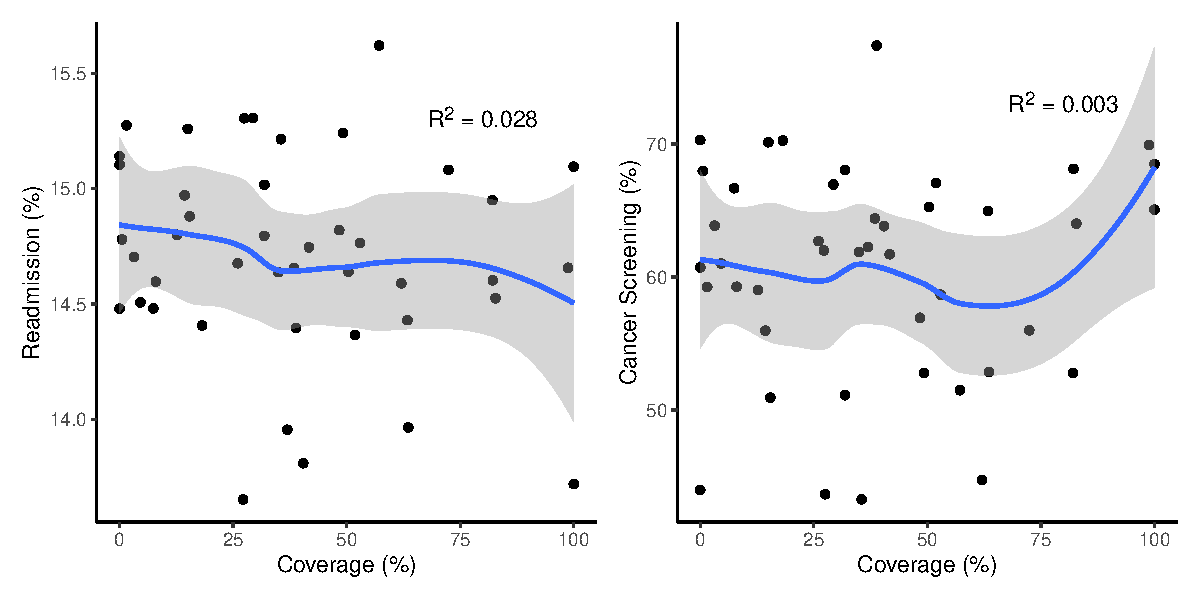
\includegraphics[width = \textwidth]{fig3-alt-1.pdf}
    \caption{The above figure show an alternative plot design to display the information in Figure 3 of \citet{basole2021}. The plot shows a scatter plot of percentage of readmission and coverage on the left and a scatter plot of percentage of cancer screening and coverage on the right. Both plots are superimposed by a local polynomial regression (displayed as a blue line) as implemented by the \texttt{loess} function in R with confidence interval for the line (displayed in gray) as implemented by the default \texttt{geom\_smooth} function in the \texttt{ggplot2} package. See Figure~S2 in the Supplementary Material for the code.}
    \label{fig:fig3-alt-with-line}
\end{figure}


\section{Making inferences from a single plot is prone to over-reading it}\label{sec:visinf}

Making a conclusion from a single plot, is analogous to making a conclusion from a single numerical summary statistic without carefully calibrating by the standard deviation. Plots are (graphical summary) statistics and thus statistical inference machinery ought to be used to assess the significance of structure seen in the plot~\citep{wickham2010graphical}. A single plot is commonly used to make inferences or assertions, however, this may result in over-reading a plot. A (data) plot can be treated as a statistic with its variation calibrated so as not to wrongfully over-emphasise an observed feature in the plot when the feature is a common artefact of random sampling. \citet{buja2009statistical} introduced the lineup protocol to calibrate a data plot by embedding it randomly among a set of null plots (a null plot has the same mapping and geometrical rendering as the data plot, using data generated under the null hypothesis of no pattern existing). The lineup protocol also adheres to a hypothesis testing framework and can be used to test for statistically significant patterns in plots. It would be recommended to remove any labels that may bias the reader because of pre-conceived notions about a problem.  Figure~\ref{fig:fig3-lineup} provides an example lineup as might be used in place of the right plot in Figure~3 from \citet{basole2021}. The null plots in Figure~\ref{fig:fig3-lineup} are generated by permuting cancer screening percentage against the other variables, thus breaking any association with coverage. If the data plot exhibits a strong association between cancer screening percentage and coverage then most observers will detect it from among the null plots. On the converse, if most observers cannot detect the data plot, then it is not significantly different to null plots, and one must conclude that there is no association between coverage and cancer screening percentage. A lineup is presented in Figure~\ref{fig:fig3-lineup} so you may use this to test if you can find a plot that appears strikingly different to others (the position of the data plot is only revealed in the Supplementary Material).

\begin{figure}[h!]
    \centering
    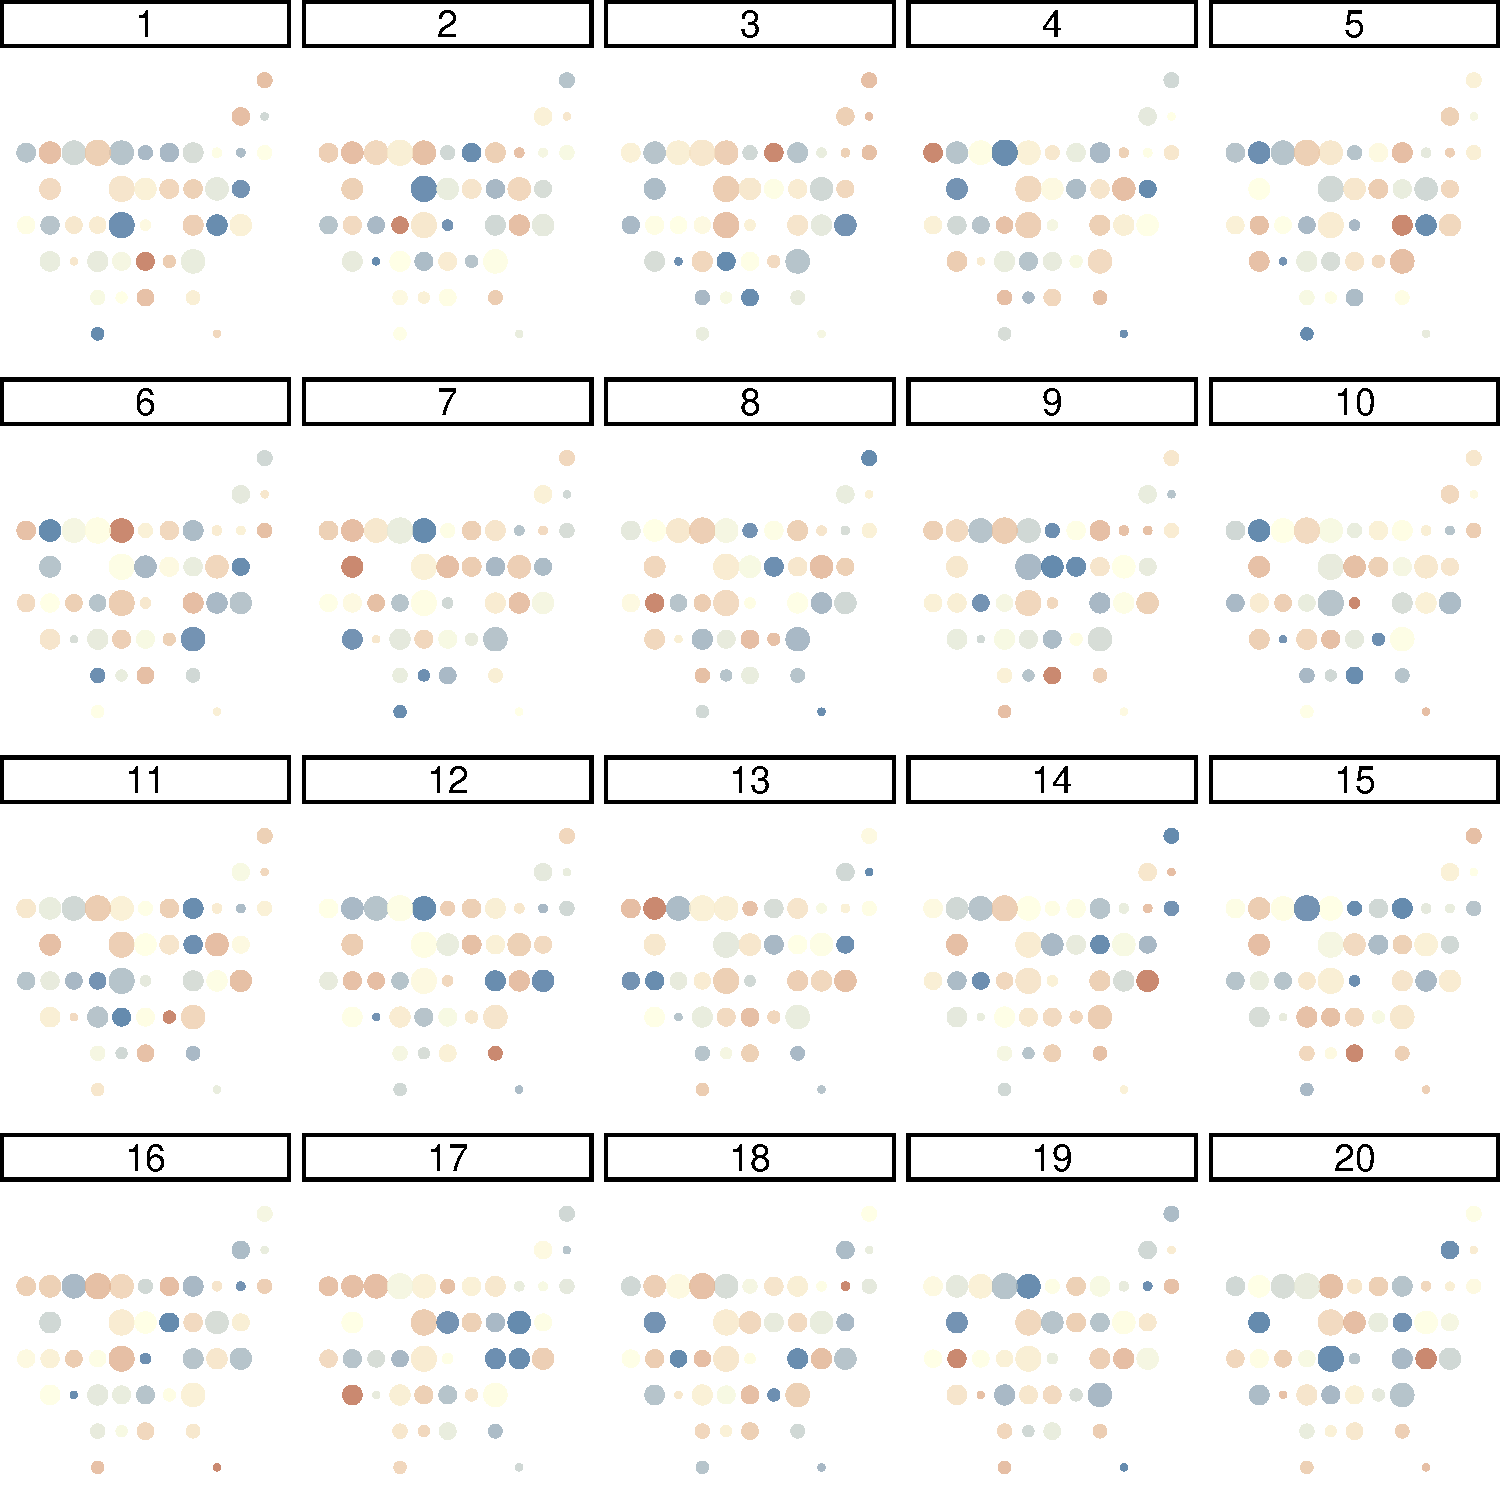
\includegraphics[width = \textwidth]{lineup-theirs-1.pdf}
    \caption{A tile grid was used in Figure 3 of \citet{basole2021} to display the cancer screening (by color) and the coverage (by size) with the tile order matching a rough spatial layout of USA. The above figure shows a lineup for this tile grid plot where one of the plots is made using the data, and the other nineteen plots are constructed after first permuting the percentage of cancer screening across different states. (Missing value structure is preserved.) Text and legends have been removed to minimise the bias in reading plots due to the reader being aware of the context. Your task is to identify any plot that is visually different from the others. See the Supplementary Material to see if you have selected the data plot as the most different, and also for the code to produce the lineup.}
    \label{fig:fig3-lineup}
    % remove 3rd one, make side-by-side
\end{figure}

The lineup protocol is a rigorous method to compare the power of different visual encodings \citep[see examples in][]{hofmann2012graphical}. The same lineup can be constructed using different visual encodings, and shown to multiple observers. The most powerful visual encoding will correspond to the data plot being detected the lineup more often. In the previous section, we advised that the scatterplot is a more powerful visual encoding, than the tile grid, for assessing association between two variables.  The Supplementary Materials has additional lineups that support this. 

%\st{Specifically, Figures~S3 and S4 can be used to compare the lineup using the tile grid plot and the scatter plot, respectively. As we do not believe there is any strong association between coverage and cancer screening percentage, we do not think the data plot can be distinguished from the null plot in the lineups shown in Figures~S3 and S4, unless, the data plot was viewed in isolation before viewing the lineups; in this case, the observer may be biased. We also include lineups for the tile grid plot and scatter plot where there is a strong association between the variables (Figures~S5 and S6). The data plot from Figures~S5 and S6 should strike out to be different to most observers, although we would argue that it is easier to spot the data plot in Figure~S6 (scatter plot) than Figure~S5 (tile grid plot).} 

\section{Final thoughts}\label{sec:conclude}

The advancements of computational subsystems, such as \texttt{ggplot2} R-package \citep{ggplot2}, \texttt{matplotlib} python library \citep{Hunter:2007} and \texttt{D3} javascript \citep{D3}, have proliferated the production of graphs in a reproducible manner. In particular, we can now generate motion graphs and, by extension, interactive graphs and dashboards very efficiently. The ease of graph production however does not assure the quality of visualisation practice.


Sub-standard visualisation practice burgeons as a result of informal treatment of plots, including over-emphasis on particular features of plots for decision-making processes. Considering plots as a statistic, treating it with the a similar rigour used to treat numerical statistics in inferences, can help in weeding out poor practices. We refer readers interested in learning more about visual inference to \cite{vanderplas2020testing}.  

%[TO DO: write more specific examples to inform readers where they can find more materials] Visual inference is a growing area \citep{buja2009statistical, wickham2010graphical, hofmann2012graphical, majumder2013validation,vanderplas2020testing,Vanderplas-Rottger-Cook-Hofmann} and we encourage adoption of these latest research to assessments of visual encoding choices.


In addition, interactive graphs and dashboards have gained significant popularity in numerous business and e-commerce applications. An interactive visualization enables us to explore the “what-if” scenarios under different assumptions and to uncover unexpected patterns under different conditions. With live data updates, dashboards are often used for visual reports of key performance indicators, enabling interactive monitoring and real-time analysis. With the abundant and complex data available, it is evermore important that visual encoding choices are chosen to communicate the intended message to the audience efficiently, but also understood without misrepresentation. We believe future research benefits from extending existing visual inference foundations to interactive graphics \citep{Cook2021Foundation} and look forward to cultivation of statistical rigour in data visualisation.  



\section*{Supplementary Materials}\label{sec:supp}

All figures in this paper are produced by using the R language \citep{rstats} and the \texttt{ggplot2} package \citep{ggplot2} are supplied at \url{https://emitanaka.org/supp-visOM/}.

% Acknowledgments here
\ACKNOWLEDGMENT{Data ethics note: the data used for the plots is synthetic data supplied by \citet{basole2021}.}

\bibliographystyle{informs2014} 
\bibliography{references} 

\end{document}







